\documentclass[12pt]{article}\usepackage[margin=1in]{geometry}\usepackage{amsmath,amssymb,amsthm,graphicx,natbib,microtype}\newtheorem{theorem}{Theorem}\newtheorem{corollary}[theorem]{Corollary}
\title{Defect-Stable Rayleigh Recurrence\\\large Additive Loewner Errors and a Sharp Affine Law}\author{Prime Dynamics Theory Program}\date{July 2026}
\begin{document}\maketitle
\begin{abstract}
Exact cross-level comparison is too rigid for validated computations.  We
prove the defect-stable form.  If $H=S^*GS$,
$G'\succeq a(1-\eta)H$, and
$D'\preceq bS^*DS+\delta H$, where $a>0$ and $0\leq\eta<1$, then
\[
 (\gamma')^2\leq\frac{b\gamma^2+\delta}{a(1-\eta)}.
\]
The bound is sharp already for scalars and gives an affine recurrence for
the squared relative tail constant.  A 4,096-instance random matrix audit
has zero failures.  This establishes robust transfer algebra but does not
prove physical all-level coefficients.
\end{abstract}
\section{The defect model}
Let $G\succ0$, $D\succeq0$, and $D\preceq\gamma^2G$.  A frame gauge gives
$H=S^*GS$.  Relative recent-Gram loss is represented by $\eta$, while an
additive tail defect is measured in the same metric $H$.  This choice is
coordinate covariant and separates geometric loss from tail forcing.

\begin{theorem}[Defect-stable transfer]\label{thm:defect}
Assume
\[
G'\succeq a(1-\eta)H,\qquad
D'\preceq bS^*DS+\delta H
\]
with $a>0$, $b,\delta\geq0$, and $0\leq\eta<1$.  Then
\[
(\gamma')^2\leq\rho\gamma^2+q,qquad
\rho=\frac{b}{a(1-\eta)},\quad q=\frac{\delta}{a(1-\eta)}.
\]
\end{theorem}
\begin{proof}
Congruence gives $S^*DS\preceq\gamma^2H$, hence
$D'\preceq(b\gamma^2+\delta)H$.  The Gram lower gives
$H\preceq G'/[a(1-\eta)]$.  Combining the inequalities and using the
variational definition of $\gamma'$ proves the claim.
\end{proof}
The argument is ordinary Loewner calculus \citep{Bhatia2007,HornJohnson1991}.

\begin{corollary}[Constant coefficients]
If $x_{n+1}\leq\rho x_n+q$, then for $\rho\ne1$,
\[
x_n\leq\rho^nx_0+q\frac{1-\rho^n}{1-\rho}.
\]
For $0\leq\rho<1$, $\limsup x_n\leq q/(1-\rho)$.
\end{corollary}

\section{Sharpness}
Take one-dimensional $G=H=1$, $D=\gamma^2$,
$G'=a(1-\eta)$, and $D'=b\gamma^2+\delta$.  Every hypothesis is an equality
and so is the conclusion.  Therefore no smaller universal coefficient of
$\gamma^2$ or $\delta$ follows from this information class.

\section{Audit and route boundary}
The audit samples 4,096 positive pairs, gauges, multiplicative constants,
Gram losses, and additive tail defects.  Targets are generated inside the
two Loewner enclosures.  There are zero hypothesis or conclusion failures,
and the scalar sharp record agrees to relative error below $10^{-12}$.
\begin{figure}[h]\centering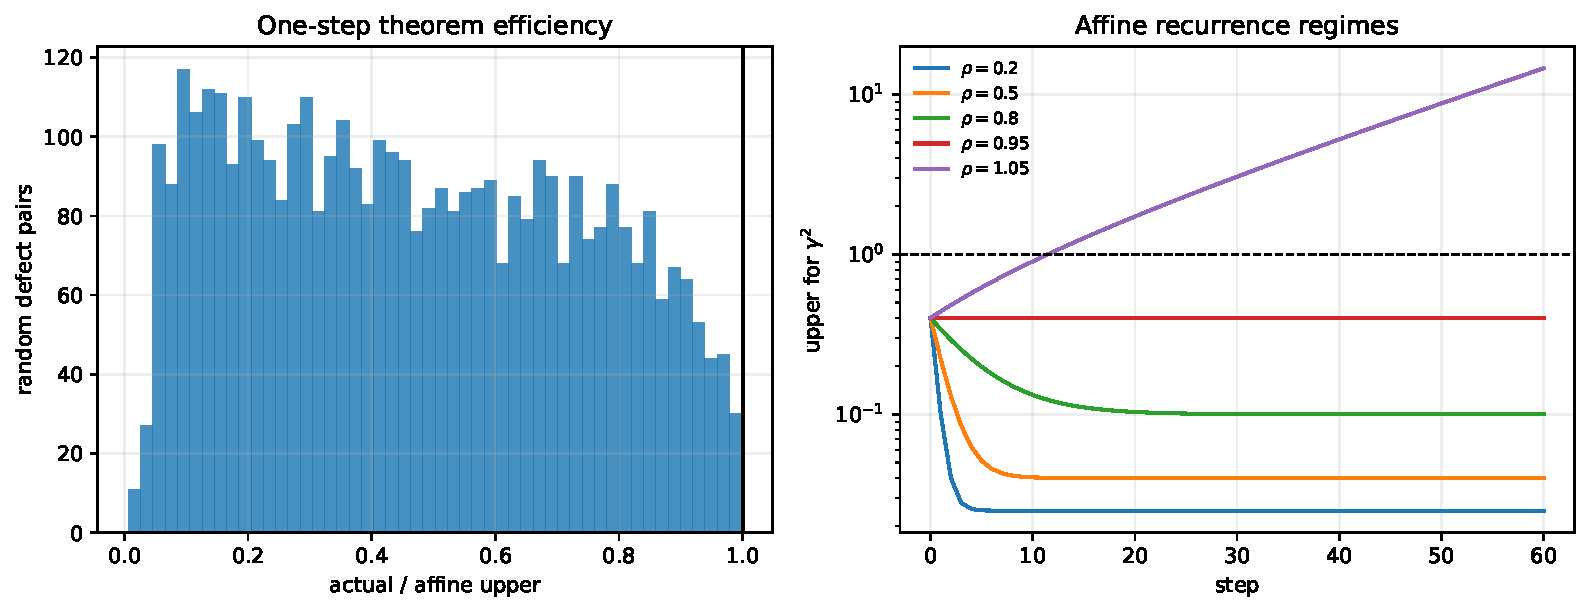
\includegraphics[width=\textwidth]{figures/defect_stable_rayleigh_recurrence.pdf}\caption{One-step efficiency and the contractive, critical, and expansive affine regimes.}\end{figure}

RH-123 supplies the recurrence form needed for outward validation.  A useful
all-level result still requires physical control with $\rho<1$ and forcing
small enough to keep the limiting gamma below one.  RH-124 next transports
normalization and capacity.  No uniform Stage A, Hilbert--Polya operator,
zeta-zero identification, or Riemann Hypothesis conclusion is claimed.
\bibliographystyle{plainnat}\bibliography{references}\end{document}
